% =====================================================================
%  Banner da XXXVI Jornada de Iniciacao Cientifica e Tecnologica da Ufes
%  Emilly Lopes das Neves | Piic 2025/2026 | protocolo 202526313
%  Modelo: poster_dmbv_Marcos_Vinicius/poster-jornada-2024.tex (LABOTIM),
%  classe baposter original (copiada para esta pasta), papel A0 retrato.
%  Compilar:  tectonic banner/banner.tex
% =====================================================================
\documentclass[portrait,a0paper,fontscale=0.285]{baposter}

% A classe carrega xcolor em cmyk, o que acinzenta os azuis; forcamos rgb.
\selectcolormodel{rgb}
\usepackage[utf8]{inputenc}
\usepackage[T1]{fontenc}
\usepackage[brazilian]{babel}
\usepackage{palatino}
\usepackage{graphicx}
\usepackage{amsmath}
\usepackage{amssymb}
\usepackage{booktabs}
\usepackage{array}
\usepackage{enumitem}
\usepackage{capt-of}
\usepackage[font=small,labelfont=bf]{caption}
\usepackage[portuguese,ruled,linesnumbered]{algorithm2e}
\usepackage{xcolor}
\usetikzlibrary{calc}

% Cores do modelo do LABOTIM (poster_dmbv_Marcos_Vinicius), medidas no PDF do lab:
% barra em degrade linear de preto a ciano, borda azul.
\definecolor{lightblue}{rgb}{0.145,0.6666,1}   % mesma definicao do modelo (#25AAFF)
\definecolor{borda}{HTML}{3189D1}              % borda como sai no PDF do modelo
\definecolor{navy}{HTML}{1C4A9E}
\definecolor{alerta}{HTML}{A33225}
\definecolor{cam1}{HTML}{E6194B}\definecolor{cam2}{HTML}{3CB44B}
\definecolor{cam3}{HTML}{4363D8}\definecolor{cam4}{HTML}{F58231}
\definecolor{cam5}{HTML}{911EB4}\definecolor{cam6}{HTML}{46F0F0}
\newcommand{\amostra}[1]{\textcolor{#1}{\rule[0.28ex]{2.0em}{0.45ex}}}
\newcommand{\fonte}{\caption*{\scriptsize Fonte: Produção da própria autora.}}
\setlist[itemize]{leftmargin=1.2em, itemsep=2pt, topsep=2pt, parsep=0pt}

\begin{document}
\begin{poster}{
headerborder=closed,
colspacing=1em,
bgColorOne=white,
bgColorTwo=white,
borderColor=borda,
headerColorOne=black,
headerColorTwo=lightblue,
headerFontColor=white,
boxColorOne=white,
textborder=roundedleft,
eyecatcher=true,
headerheight=0.11\textheight,
headershape=roundedright,
headershade=plain,
headerfont=\Large\bf\textsc,
linewidth=2pt
}
% ------------------------------------------------- eyecatcher (esquerda)
{
\includegraphics[height=10em]{logos/labotim-ufes.png}}
% ------------------------------------------------------------- titulo
{{\LARGE\bfseries Otimização Dinâmica de Rotas para Coleta de Resíduos\\[0.1em] Sólidos: Adaptação do Algoritmo de Solomon com Integração IoT}\vspace{0.3em}}
% ------------------------------------------------------------ autores
{Emilly Lopes das Neves e Maria Claudia Silva Boeres \hspace{12pt}\\
 Universidade Federal do Espírito Santo \quad $\cdot$ \quad \textbf{Protocolo 202526313}}
% ------------------------------------------------------ logo (direita)
{
\includegraphics[height=10em]{logos/fapes-cor.png}}

% O Tectonic nao renderiza o shading nativo do baposter: o degrade da barra de
% titulo e emulado com 60 faixas solidas, e a ultima leva o canto arredondado.
\makeatletter
\newcommand{\baposterFaixas}{%
  \foreach \i in {0,...,59}{%
    \pgfmathsetmacro{\pa}{\i*100/59}\colorlet{faixa}{lightblue!\pa!black}%
    \path[fill=faixa]
      let \p1=(\baposter@box@name tnw), \p2=(\baposter@box@name ne),
          \n0={\x2-\baposter@box@@cornerradius},
          \n1={\x1+(\n0-\x1)*(\i/60)}, \n2={\x1+(\n0-\x1)*((\i+1)/60)+1pt}
      in (\n1,\y1) rectangle (\n2,\y2);
  }%
  \path[fill=lightblue]
    let \p1=(\baposter@box@name tnw), \p2=(\baposter@box@name ne),
        \n0={\x2-\baposter@box@@cornerradius}, \n3={\baposter@box@@cornerradius}
    in (\n0-1pt,\y1) -- (\n0-1pt,\y2) -- (\n0,\y2) arc[start angle=90,end angle=0,radius=\n3]
       -- (\x2,\y1) -- cycle;}
% headershade=plain chama esta macro ja com as coordenadas da caixa definidas:
% desenhamos as faixas aqui e deixamos a barra original so com o contorno.
\renewcommand{\baposter@box@headershade@plain}[3]{%
  \baposterFaixas\tikzstyle{header colors}=[draw=#3,fill=none]}
\makeatother

% ====================================================== RESUMO ========
\headerbox{\normalsize Resumo}{name=resumo,column=0,row=0,span=3}{
Este subprojeto comparou \textbf{cinco heurísticas clássicas} para o Problema de
Roteamento de Veículos com Janelas de Tempo (VRPTW), todas sobre o mesmo núcleo
de código: a inserção I1 de Solomon, a Descida em Vizinhança Variável (VND), o
GRASP nas formas fixa e reativa e a Busca Tabu. Nas \textbf{56 instâncias de
Solomon}, com calibração pelo \textit{irace} e testes de Friedman e Wilcoxon, as
variantes de GRASP ficaram \textbf{abaixo de 2\,\% do melhor conhecido}, sem
nenhuma solução inviável. Um \textbf{gêmeo digital} levou o GRASP à coleta
seletiva de Vitória/ES, com sensores de nível simulados: a coleta sob demanda
\textbf{reduziu as coletas em 46\,\%} com distância comparável.
}

% ===================================================== RODAPE =========
% Definido antes das colunas: no baposter, above= exige a caixa ja criada.
\headerbox{\normalsize Agradecimentos}{name=agradecimento,column=0,above=bottom,span=2,height=0.085}{
Agradeço à professora Maria Claudia Silva Boeres (UFES-CT) e ao professor Renato
Elias Nunes de Moraes (UFES-CT), por coordenar e orientar este projeto; ao Piic/Ufes,
pela bolsa; e à Fapes (projeto n.\textsuperscript{o} 2026-6NX7B), pelo apoio financeiro a esta pesquisa.
}

\headerbox{\normalsize Referências}{name=references,column=2,above=bottom,height=0.085}{
\scriptsize
[1] SOLOMON, M. M. \textit{Operations Research}, v.~35, 1987.\par
[2] FEO, T.; RESENDE, M. \textit{J. Global Optim.}, v.~6, 1995.\par
[3] GLOVER, F. \textit{ORSA J. Computing}, v.~1, 1989.\par
[4] LÓPEZ-IBÁÑEZ, M. et al. \textit{ORP}, v.~3, 2016.\par
[5] DEM\v{S}AR, J. \textit{JMLR}, v.~7, 2006.
}

% ==================================================== COLUNA 0 ========
\begin{posterbox}[name=problema,column=0,below=resumo]{O problema}
A coleta urbana segue \textbf{rotas e frequências fixas}, qualquer que seja o
conteúdo da lixeira. Isso gera \textbf{visitas inúteis} (esvaziar lixeira quase
vazia) e \textbf{transbordos} (a lixeira enche antes da visita). Sensores de
nível em rede LoRaWAN permitem coletar \textbf{só o que precisa}, mas o plano
de rotas tem de ser refeito a cada ciclo e continuar viável.

\vspace{0.3em}
\textit{Qual heurística clássica sustenta esse replanejamento com qualidade e
sem violar as janelas de tempo?}
\end{posterbox}

\begin{posterbox}[name=vrptw,column=0,below=problema]{O VRPTW}
Uma frota de capacidade $Q$ sai de um depósito e visita cada cliente uma única
vez, dentro da sua \textbf{janela de tempo} $[e_i,\ell_i]$ e sem exceder a carga
do veículo:
\[
  b_i \le \ell_i \ \ \forall i, \qquad \textstyle\sum_{i\in r} q_i \le Q .
\]
O objetivo é minimizar a \textbf{distância total} percorrida. O \textbf{gap} é
a distância percentual entre a solução obtida e a melhor conhecida da instância:
quanto menor, melhor.
\end{posterbox}

\begin{posterbox}[name=metodos,column=0,below=vrptw]{Os cinco métodos}
\begin{tabular}{@{}p{0.36\linewidth}@{\ }p{0.62\linewidth}@{}}
\textbf{I1 de Solomon} & inserção gulosa; ponto de partida de todos.\\
\textbf{VND} & seis vizinhanças em ordem fixa.\\
\textbf{GRASP} & construção aleatória ($\alpha$) mais VND, repetida.\\
\textbf{GRASP reativo} & aprende o melhor $\alpha$ durante a busca.\\
\textbf{Busca Tabu} & aceita pioras e proíbe desfazer movimentos.\\
\end{tabular}

\vspace{0.4em}
Todos foram escritos em C++20 sobre o \textbf{mesmo núcleo de código}, então a
estratégia de busca é a única origem das diferenças.
\end{posterbox}

\begin{posterbox}[name=conclusao,column=0,below=metodos,above=agradecimento]{Conclusões}
\begin{itemize}
  \item Hierarquia estatisticamente significativa: \textbf{GRASP $\approx$
        reativo $\succ$ Tabu $\succ$ VND $\succ$ I1}. A busca local é a maior
        contribuição isolada.
  \item No cenário de Vitória, a coleta sob demanda faz \textbf{46\,\% menos
        coletas} com rotas sempre viáveis; o limiar $\tau$ regula o
        equilíbrio entre economia e transbordos.
  \item \textbf{Próximos passos:} piloto com sensores reais e estimativa de
        custos e emissões.
\end{itemize}
\end{posterbox}

% ============================================= COLUNAS 1 e 2 ==========
\begin{posterbox}[name=metodologia,column=1,below=resumo,span=2]{Metodologia}
\begin{minipage}[t]{0.47\textwidth}
\vspace{0pt}
\textbf{Instâncias.} As 56 de Solomon, com 100 clientes, divididas em
\textbf{28 de treino} (calibração) e \textbf{28 de teste} (comparação), para que
nenhum método seja avaliado em dados que já viu.

\vspace{0.4em}
\textbf{Calibração.} O \textit{irace} ajustou o $\alpha$ do GRASP e a
\textit{tenure} da Tabu; o valor calibrado só entrava se vencesse o clássico
no teste. Todos param após \textbf{800 iterações sem melhora}.

\vspace{0.4em}
\textbf{Validação.} Um verificador independente recalcula cada solução final:
\textbf{3.528 execuções, nenhuma inviável}.

\vspace{0.4em}
\textbf{Estatística.} Teste de Friedman e Wilcoxon pareado com correção de
Holm, a 5\,\%.
\end{minipage}
\hfill
\begin{minipage}[t]{0.50\textwidth}
\vspace{0pt}
\small
\begin{algorithm}[H]
\caption{GRASP com VND}
\SetAlgoLined
\Entrada{instância, $\alpha=0{,}30$, $K=800$}
\Saida{melhor solução $S^\star$}
$S^\star \gets$ I1-Solomon(instância); $k \gets 0$\;
\Enqto{$k<K$}{
  $S \gets$ Construção-Aleatória($\alpha$)\;
  $S \gets$ VND($S$)\;
  \eSe{$D(S) < D(S^\star)$}{$S^\star \gets S$; $k \gets 0$\;}{$k \gets k+1$\;}
}
\Retorna{$S^\star$}
\end{algorithm}
\end{minipage}
\end{posterbox}

\begin{posterbox}[name=resultados,column=1,below=metodologia,span=2]{Resultados nas instâncias de Solomon}
\begin{minipage}[t]{0.47\textwidth}
\centering
\captionof{figure}{\small Gap médio ao melhor conhecido (escala log).}
\vspace{-0.4em}
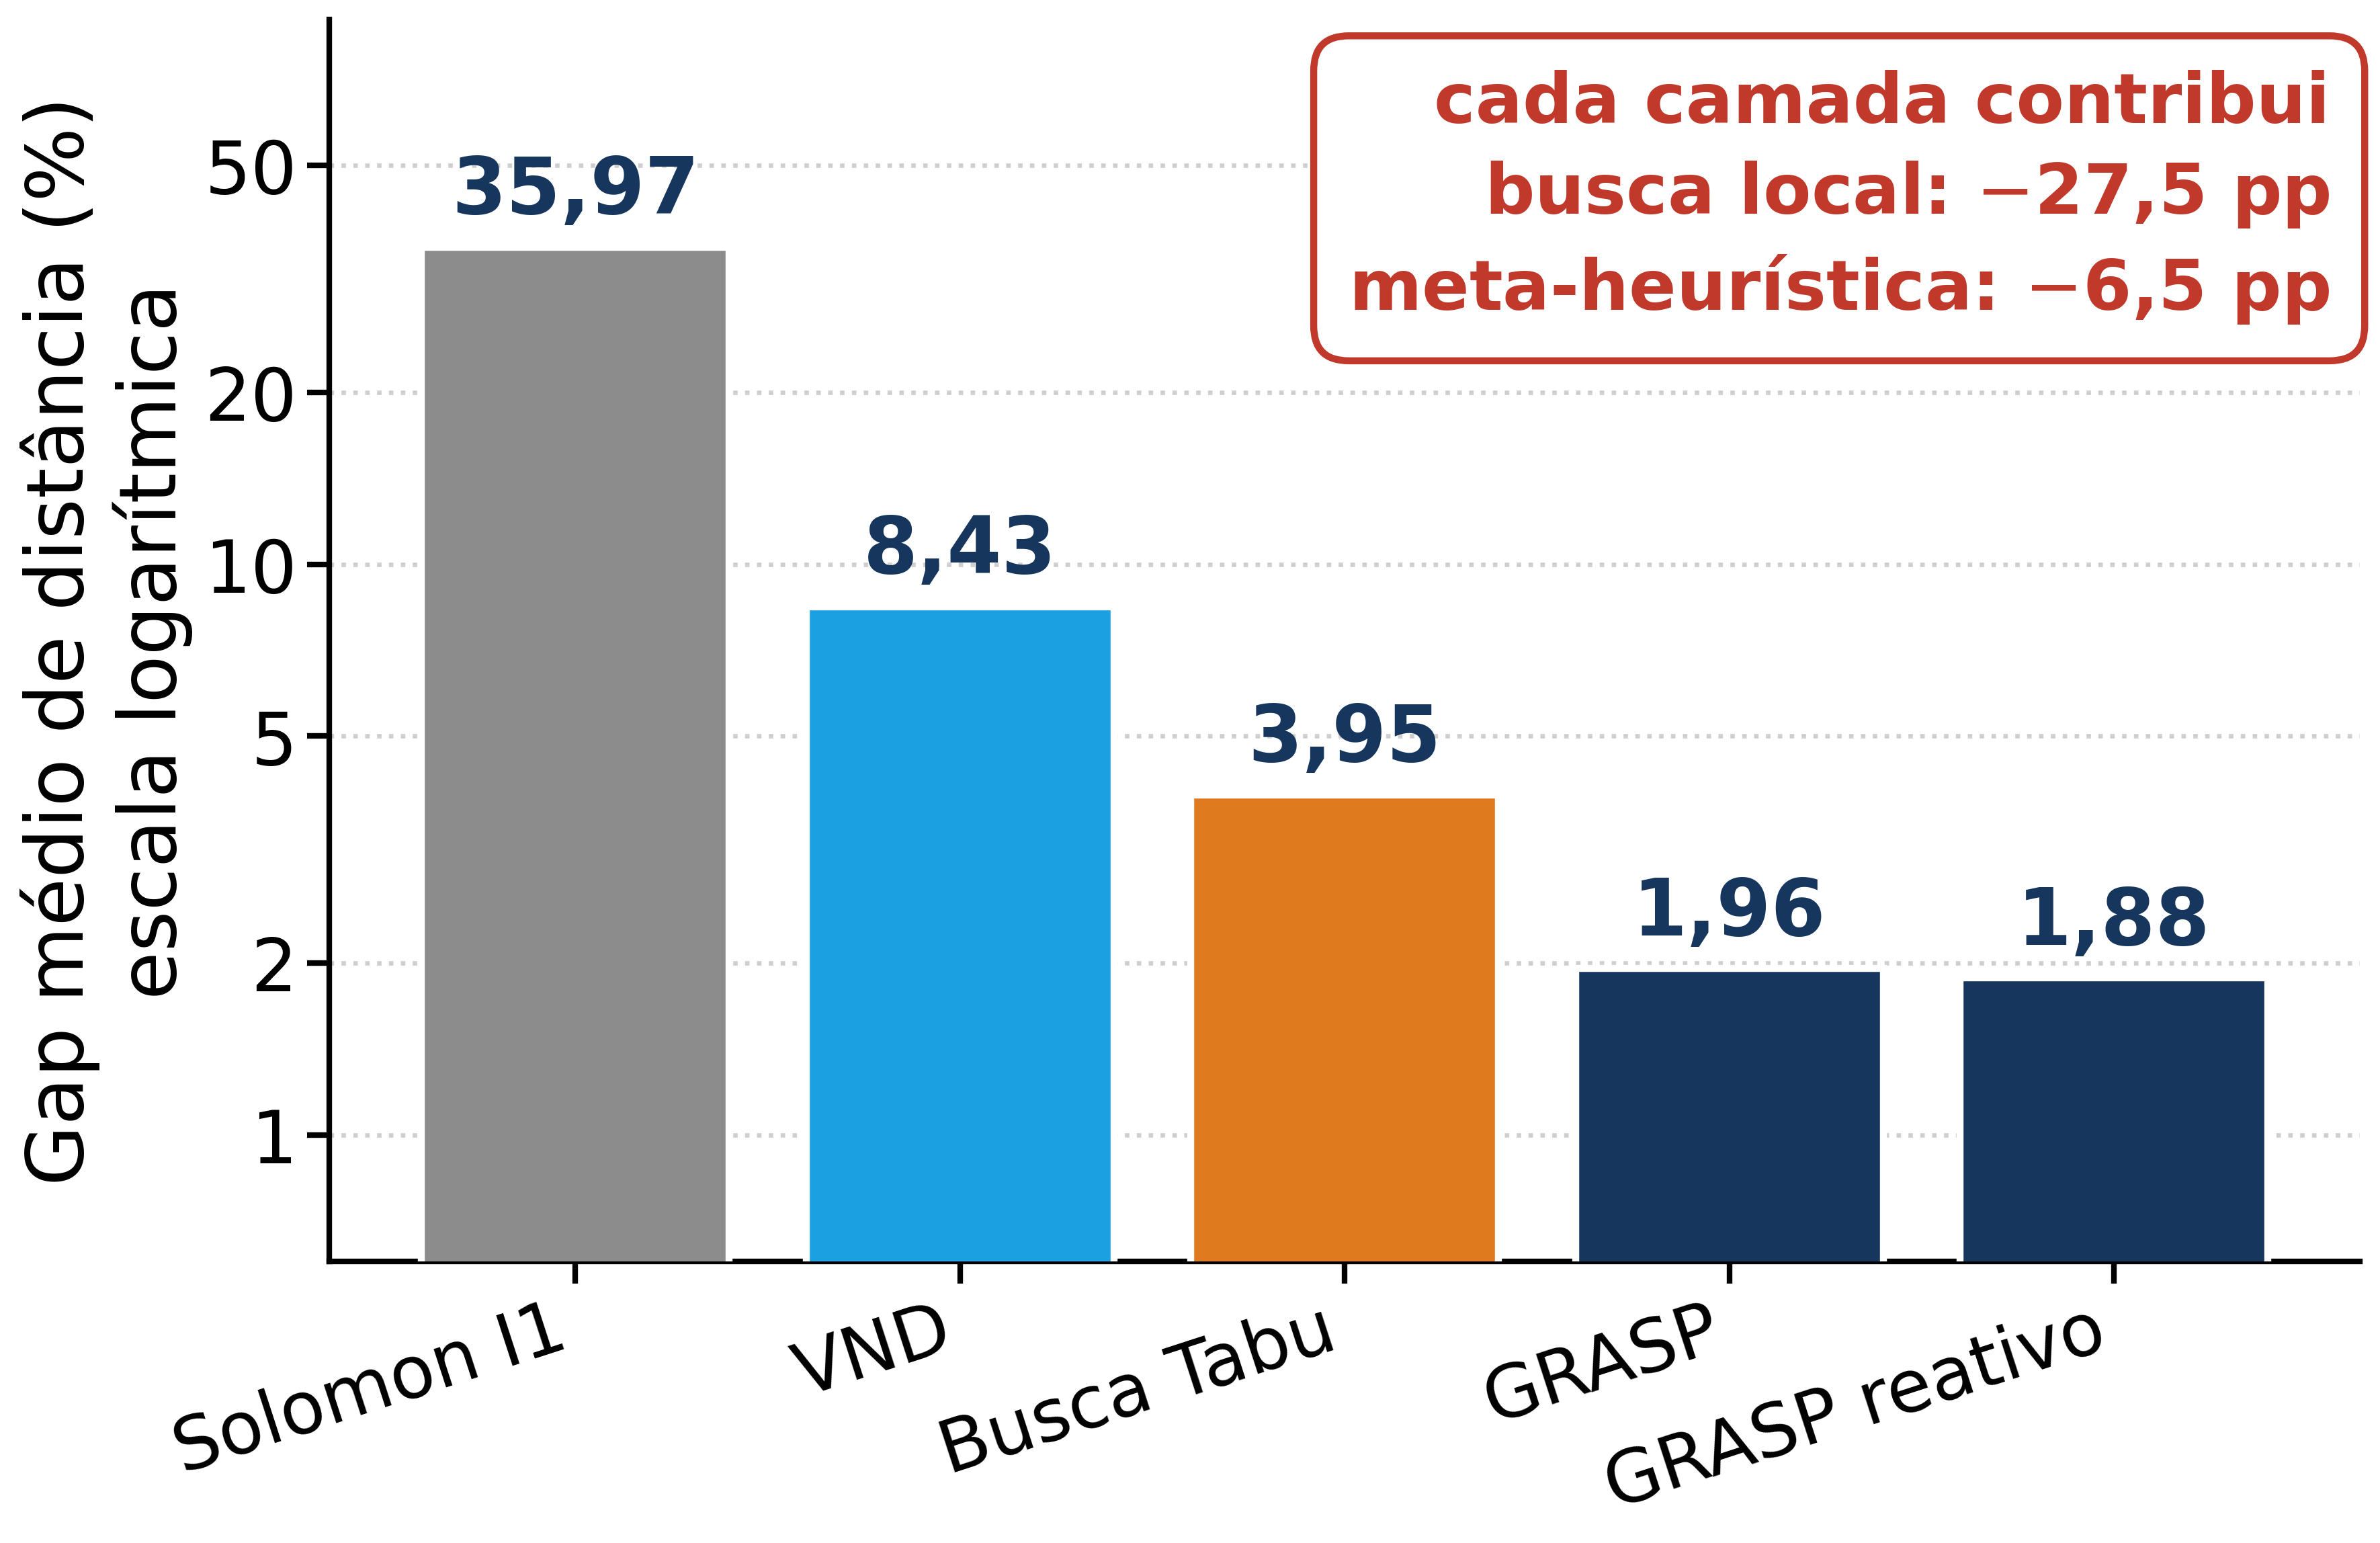
\includegraphics[width=\linewidth]{figuras/cascata_gap.png}
\fonte
\end{minipage}
\hfill
\begin{minipage}[t]{0.50\textwidth}
\centering
\captionof{figure}{\small Posto médio de cada método (menor é melhor); a barra une os que não diferem.}
\vspace{-0.4em}
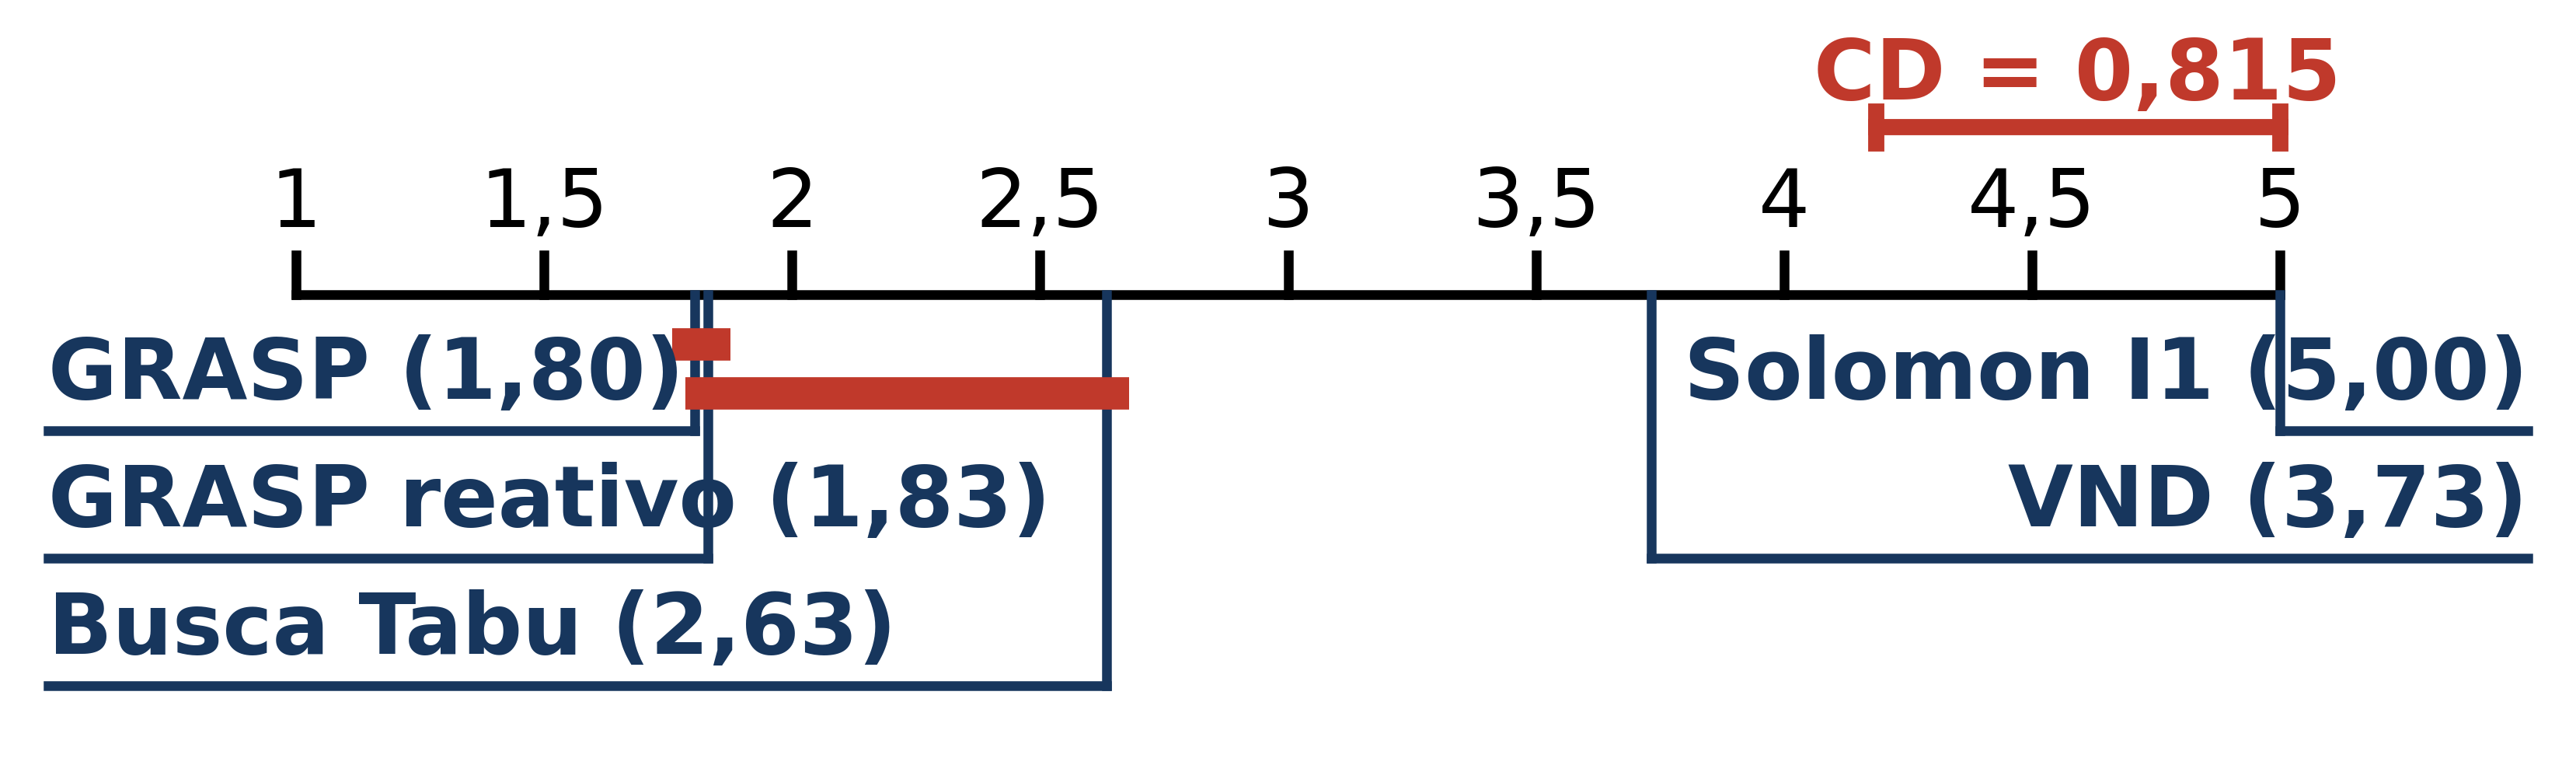
\includegraphics[width=\linewidth]{figuras/cd_diagrama.png}
\fonte

\vspace{0.5em}
\raggedright
Cada camada reduz o gap: \textbf{36\,\%} na I1, \textbf{8,4\,\%} com o VND e
\textbf{1,9\,\%} no GRASP. Nas 28 de teste, Friedman rejeita a igualdade
($p = 1{,}7\times10^{-19}$) e o Wilcoxon separa todos os pares, exceto GRASP e
reativo.
\end{minipage}
\end{posterbox}

\begin{posterbox}[name=twin,column=1,below=resultados,span=2,above=agradecimento]{Gêmeo digital da coleta seletiva de Vitória}
\begin{minipage}[t]{0.46\textwidth}
\vspace{0pt}
\centering
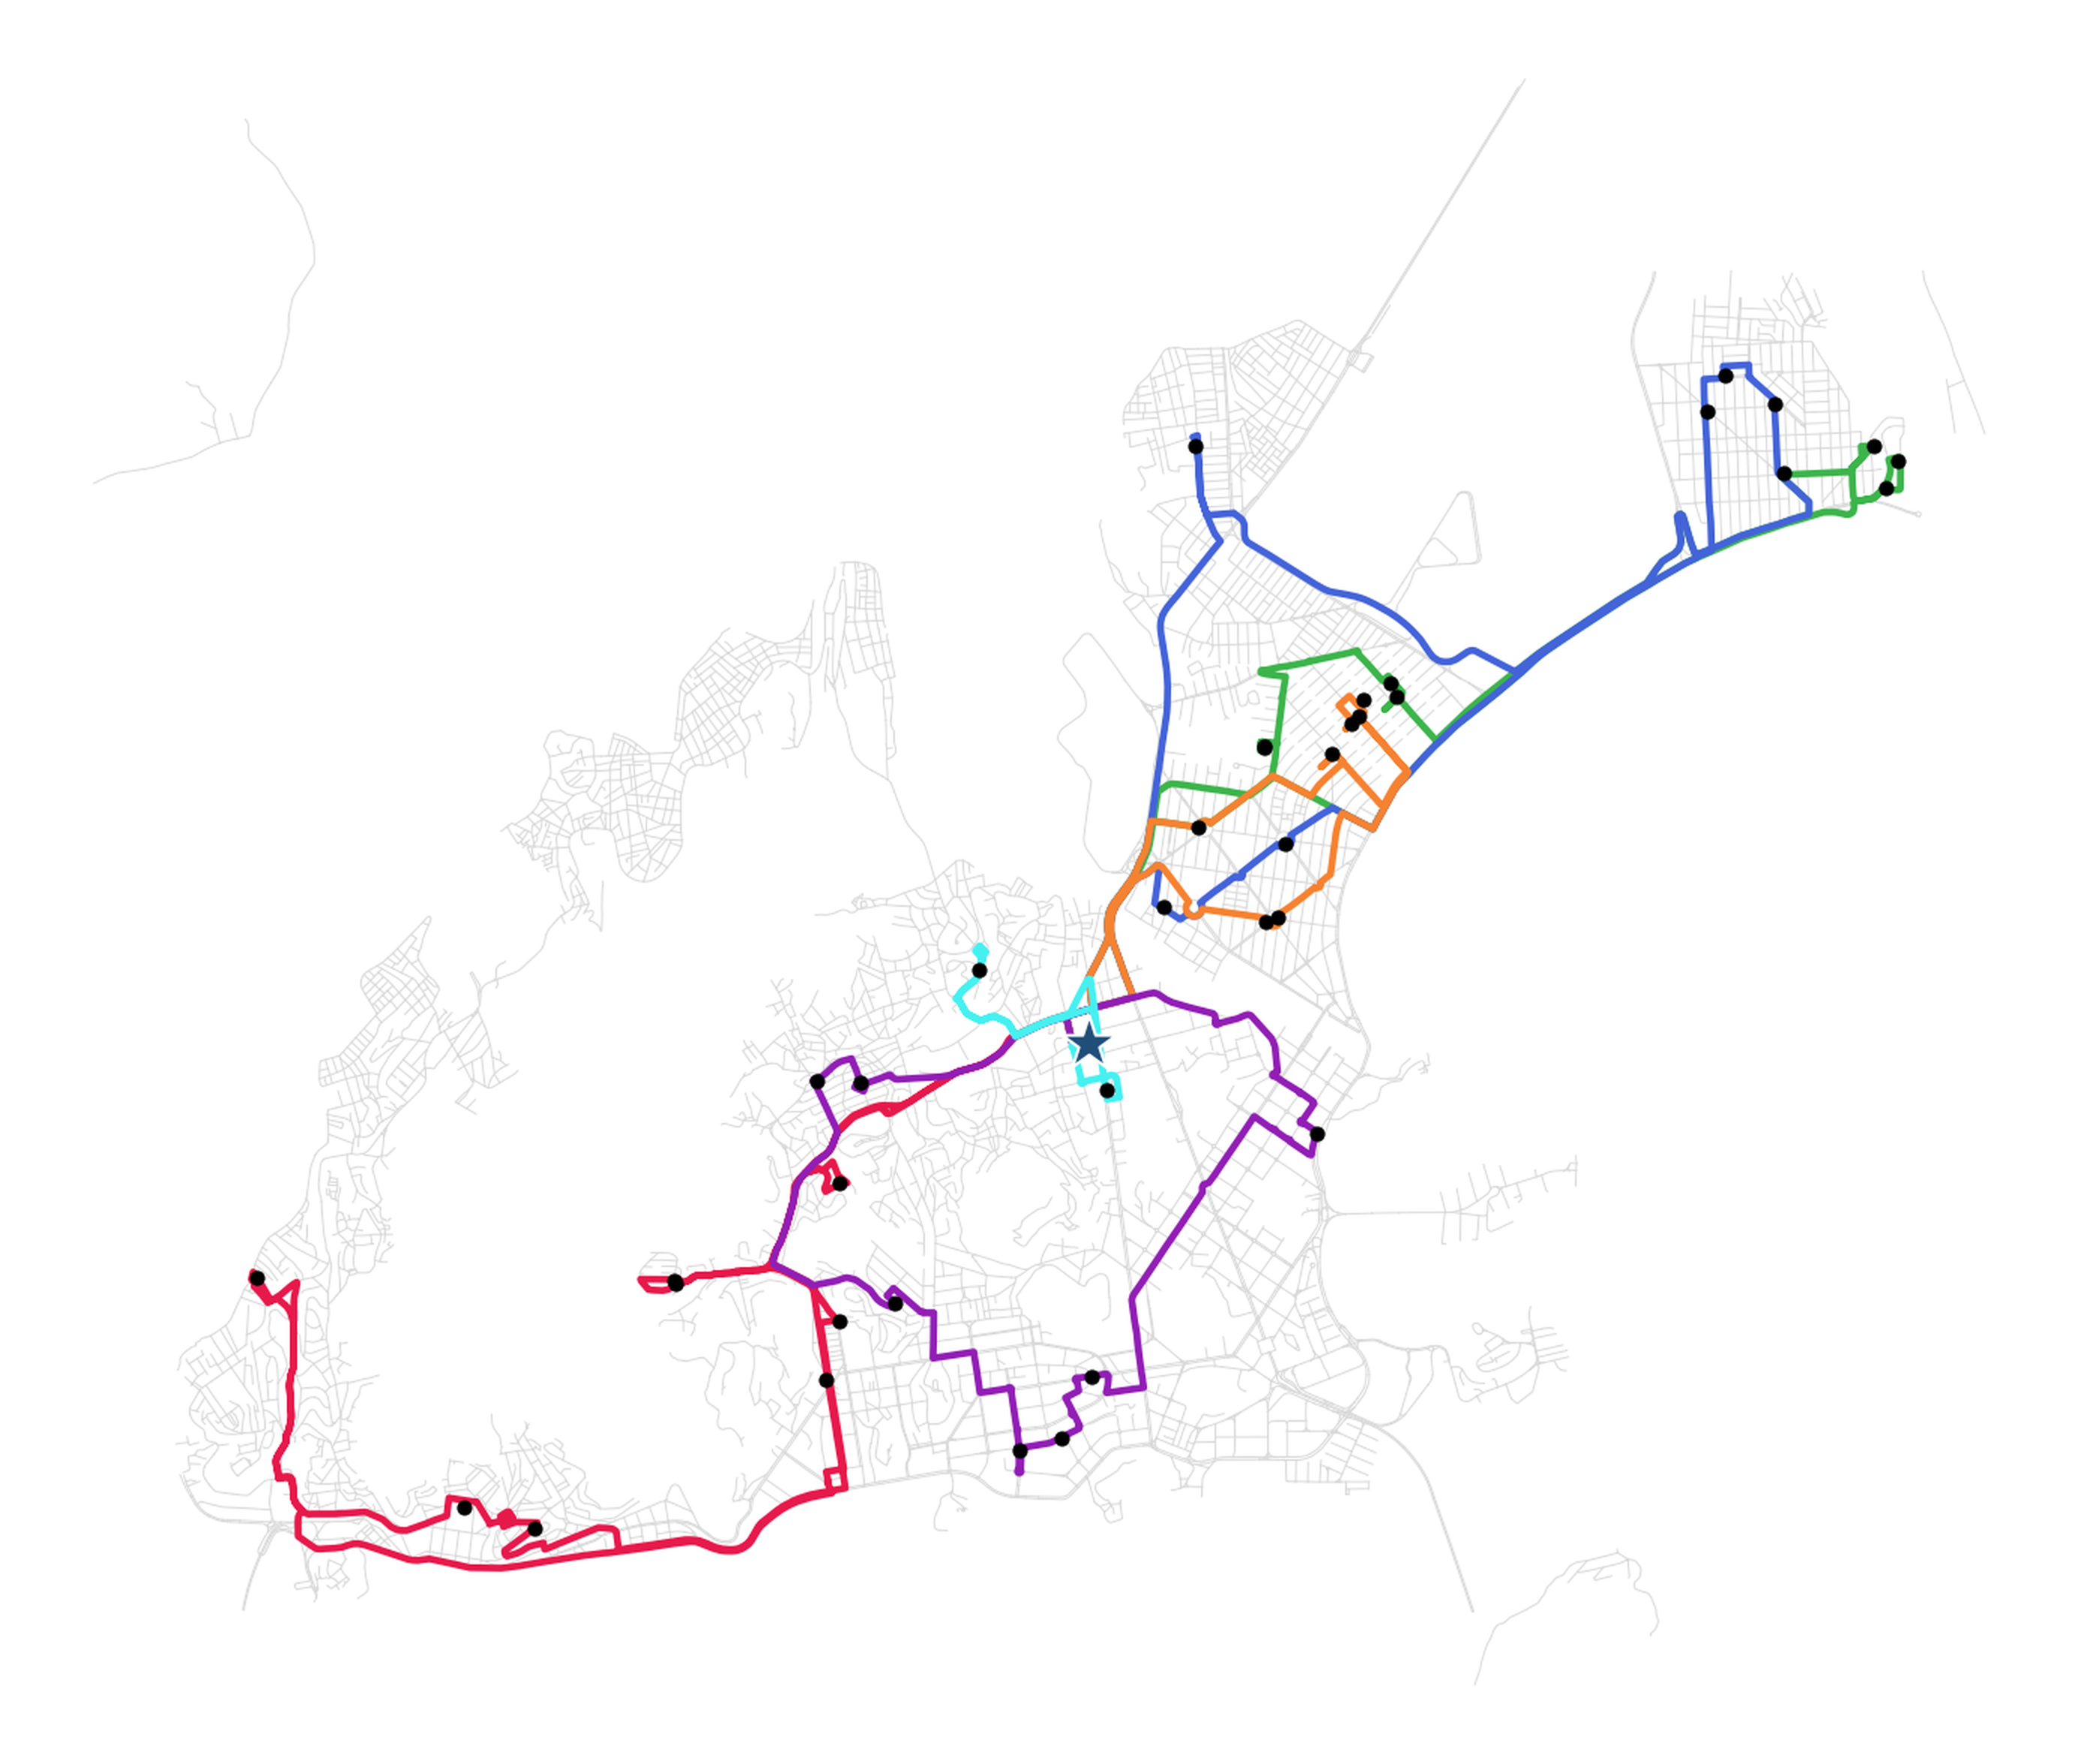
\includegraphics[width=0.97\linewidth]{figuras/mapa_vitoria.png}\\[0.1em]
{\footnotesize
\begin{tabular}{@{}l@{\ }l@{\quad}l@{\ }l@{\quad}l@{\ }l@{}}
\amostra{cam1} & Caminhão 1 & \amostra{cam3} & Caminhão 3 & \amostra{cam5} & Caminhão 5\\
\amostra{cam2} & Caminhão 2 & \amostra{cam4} & Caminhão 4 & \amostra{cam6} & Caminhão 6\\
\end{tabular}}
\captionof{figure}{\small Rotas dos 38 pontos de coleta na malha viária real: 6 caminhões, 83,8 km.}
\end{minipage}
\hfill
\begin{minipage}[t]{0.51\textwidth}
\vspace{0pt}
\textbf{Como funciona.} O enchimento das 38 lixeiras é simulado e lido por
sensores LoRaWAN. A cada ciclo, só as lixeiras acima do limiar
$\tau = 0{,}7$ entram no plano, e o GRASP gera as rotas. O regime
\textbf{estático} coleta todas a cada 3 ciclos.

\vspace{0.5em}
\centering
\captionof{table}{\small Médias de 30 simulações pareadas, 16 ciclos.}
\vspace{-0.3em}
\begin{tabular}{@{}lrrr@{}}
\toprule
\textbf{Regime} & \textbf{Distância} & \textbf{Coletas} & \textbf{Transbordos}\\
\midrule
Dinâmico & 3751 & \textbf{124} & 27\\
Estático & 3664 & 228 & \textbf{19}\\
\bottomrule
\end{tabular}

\vspace{0.6em}
\raggedright
\textbf{\textcolor{alerta}{Nenhum regime domina o outro.}} O dinâmico faz
\textbf{46\,\% menos coletas} com distância só 2,4\,\% maior, mas transborda
mais. O limiar é a alavanca: com $\tau = 0{,}5$, os transbordos caem para
\textbf{5} e as coletas ficam em 167, ainda bem abaixo das 228.
\end{minipage}
\end{posterbox}

\end{poster}
\end{document}
